\chapter{Business Modelering}\label{ch:businessanalysis}

I dette afsnit bliver der fokuseret på Business modeling aktiviteten under Unified Process\cite{UnifiedProcess}. Denne aktivitet indgår under Inception fasen, som skal danne et scope, samt business case. Dette tilnærmer sig et overblik over hvor projektet bærer hen ad, hvori der vil introduseres en undersøgelse af hvilke Use Cases der skal integreres i systemet. 

Business modelering indebærer en forståelse for målene for organisationen (en business analyse), som vil hjælpe til med at finde brugbare informationer omkring, hvad der skal inkluderes i systemet\cite{UP}. Ved at analysere organisationen og dens process kan gruppen herfra finde ud af, hvilke centrale Use Cases der er, hvorefter det er muligt at opstille krav til disse. Samtlige beskrivelser omkring virksomheden er enten referet til med kilde, eller er fra interviewet med Hjem-IS (se bilag \ref{app:interview}).

Hjem-IS er en af de få specialforretninger tilbage i Danmark. Virksomheden er grundlagt på, at sælgere kører ud på de forskellige ruter tildelt. Hjem-Is kom til Danmark i 1976\cite{Hjemisabout}, efter at svenskeren Eric Ericsson først bragte ideen til livs i sverige ved at spænde en fryseboks bag på sin bil, hvor han ringede med klokken, for at informere folk om at is-bilen er til stede. For i dag at kunne holde virksomheden igang kræves der god planlægning ift. hvor man skal køre og ringe med klokken, hvilke produkter man skal have på lager og hvor mange, og samtidig kunne håndtere specialordre. Der er meget planlægning og informationer, der skal holdes styr på og optimeres så alle kunderne kan få deres IS. Det betyder at der kræves pålideligt styringssoftware til at håndtere disse opgaver. 

\section{Evaluering af organisationsstruktur}
Figur \ref{fig:global_hierarchy} er et organisationsdiagram ud fra linje-stabsprincippet\cite{Organisation} og viser hierarkiet over organisationen. Den kan konkluderes til at være relativ flad, da der kun er tre lag. Ud fra givne informationer ses det, at Torben Meng er administrerende direktør og har højeste stilling, næst er der 15 ansatte på hovedkontoret, hvori Torben Meng er inkluderet.

\begin{landscape}
    \begin{figure}[p]
        \centering
        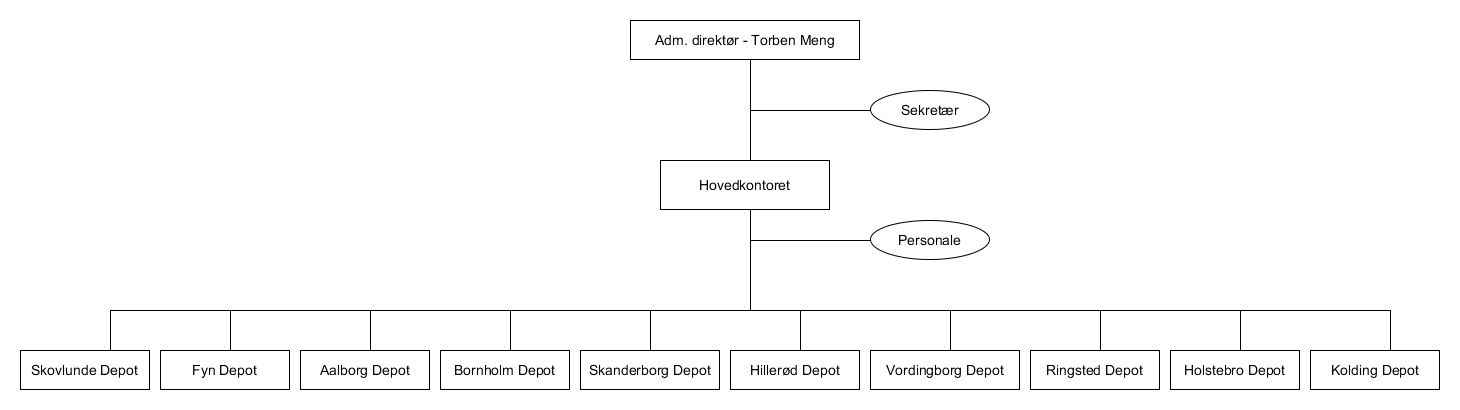
\includegraphics[width=\hsize]{figures/businesscase/global_hierarchy.png}
        \caption{Linje-stabsprincippet over hele Hjem-IS}
        \label{fig:global_hierarchy}
    \end{figure}        
\end{landscape}

Hjem-is har 165 ansatte spredt ud over 10 depoter i hele danmark, hver depot har en depotchef, som styre depotet og områderne i nærheden af Hjem-is depotet. f.eks så har aalborg depot ansvaret for at køre is rundt i hele nordjylland. Da det ikke har været muligt at interviewe og få et bedre overblik over alle depoterne hos hjem-Is er det valgt, at der fokuseres udelukkende på Aalborg depot, hvori et interview med chefen fra depotet har fundet sted. Nedenfor ses figur \ref{fig:local_hierarchy} som viser strukturen for Aalborg depotet. 

\begin{figure}[H]
    \centering
    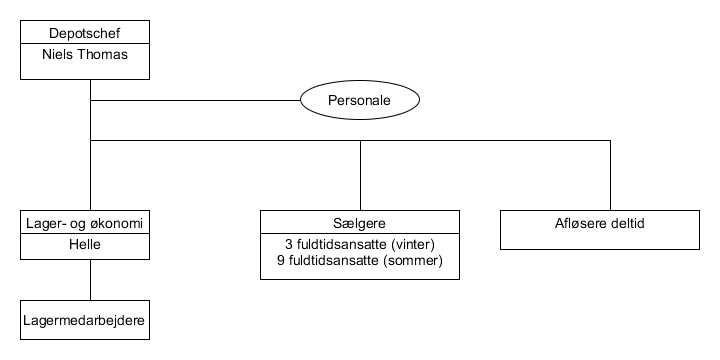
\includegraphics[width=\textwidth]{figures/businesscase/local_hierarchy.png}
    \caption{Lokal organisations hierarchy}
    \label{fig:local_hierarchy}
\end{figure}

Figur \ref{fig:local_hierarchy} viser hierarkiet for Hjem-is, igen ud fra linje-stabsprincippet\cite{Organisation}, i Aalborg depotet. Her kan det også konkluderes, at den hos depotet også er relativ flad, når det gælder strukturen. Under et interview med depotchef Niels Thomas blev det klargjort, at hos Aalborg depot er organisationsstrukturen enkelt og uformel. Der er kun 2 niveauer, depotchef Niels Thomas og så resten af medarbejderne. Afløsere er behandlet på samme måde, som fuldtidsansatte, og har de samme fordele. Oftest kan problemet med en flad organisationskultur betyde, at medarbejderne ikke er sikre på hvem de kan gå til, ift. problemer og skabe usikkerhed og tvivl. Det er ikke tilfældet, på depotet i Aalborg. På Aalborg depotet er det blevet oplyst af medarbejdere, at det et rart sted at være og at man ved hvem man kan gå til. Der er et godt forhold, mellem medarbejdere og chef. Der ses ingen ustabilitet, når det gælder tryghed for jobbet. Ud fra denne struktur, samt det forhold der er mellem medarbejdere og leder, kan der laves et kvalificeret gæt til, hvilken kulturtype der er hos Hjem-IS.

\section{Kulturtype}
Hos depotet i Aalborg, vurderes kulturtypen til at høre ind under “familien” af de fire kulturtyper\cite{Organisation}. Selvom det ikke er en hierarkisk opdeling, ligger magten stadig på depotchefens skuldrer. Fokuset er, at glæde medarbejderne bedst muligt og sørge for alle har det godt på jobbet. Det er endda tilladt at tage venner, kærester og familie med ud og køre i isbil. Der er tætte og gode relationer mellem medarbejdere. Chefen er på den anden side ikke bange for at slå med pisken, hvis en medarbejder gør skade på bilen, men hurtigt til at lave sjov med det kort tid efter. Dog hvis dette sker forventes det af medarbejderne at oplyse chefen om, hvis noget er gået galt. Herfra et meget personorienteret depot.

\section{Organisationskulturen hos Hjem-Is}
Hos depotet i Aalborg, udøves ledelsen med nem kommunikation til alle, specielt nye ansatte. Kommunikationen mellem alle på depotet er nem. f.eks, hvis en afløser gerne vil have fat på chefen, er det nemt at hoppe ind på kontoret, ringe eller skrive en sms til chefens arbejdstelefon. Herunder gives der opdateringer via mails på hvordan tallene ser ud, hvad der bliver solgt bedst og andre relevante informationer. \\
Hos depotet i Aalborg kommer succes for det meste fra den enkelte sælger. Når en sælger kommer tilbage til depotet med et godt salg, som selvfølgelig afhænger af hvilken sæson sælgeren er ude og sælge is i, får sælgeren også ros. Et typisk succesfuld salg om vinteren ligger omkring de 4000 kr, hvorimod om sommeren kan det være alt fra 8000 kr, som er set som et godt salg. Men en virkelig succesfuld dag ville typisk ramme over 10000 kr. En sælger der kommer hjem, med et meget succesfuldt salg bliver ofte belønnet med en pakke is, eller typisk en personlig sms fra depot chefen, hvori man bliver rost for salget. Det ses også, at chefen ringer ud til sælger, midt i en salgs rute for at rose eller belønne, hvis de har gjort et godt stykke arbejde. Dette medfører god og positiv energi gennem depotet, som bygger over i, at både sælgere og nye ansatte bliver motiveret til at udgøre et godt stykke arbejde. Det må aldrig blive kedeligt ude ved depotet, derfor sørger Niels Thomas for. Der skabes konkurrence mellem sælgerne, ved ofte at udgive belønninger til dagens, ugens eller månedens bedste slag. Der er et godt forhold mellem sælgere ude på depotet, når dagens er ved at komme en en ende, kassen tælles op og alle isbiler er kørt hjem, bliver der hygge-chattet mellem sælgerne, hvori dagens ture ofte bliver diskuteret frem og tilbage. Under oplæringen af afløsere/sælger, forventes det, at afløseren hurtigt lærer systemet at kende, fordi de netop er unge og hurtigt kan adaptere sig til nye systemer. Allerede på første oplærings dag, skal personen være forberedt på at køre isbilen, kende til systemet og have gjort sit første salg, med en mere erfaren medarbejder som overværer den nye medarbejder. Med denne organisationskultur kan det bestemmes at virksomhedens værdier og normer befinder sig meget ovre i fokus på glade medarbejdere.

\section{Hofstede}
Sammenholdet i organisationskulturen hos Hjem-is kan beskrives med Hofstede og hans teorier, herunder Hofstede dimensions of organisational culture. Der er 6 dimensioner: Means- vs Goal-oriented, Internally vs Externally Driven, Easygoing vs Strict Work Discipline, Local vs Professional, Open vs Closed System, Employee-oriented vs Work-oriented\cite{Quickbase}. Disse dimensioner kan bruges til at skabe sig et overblik over hvordan firmaets egentlige kultur er, samt hvilken kultur de måske ønsker sig, samt om virksomheden er klar til ændringer og på hvor stort et plan de er det. Den ønskede kultur hos Hjem-IS er at alle udfører opgaverne og opnår målene, samt har det sjovt og godt på arbejdet. Det er en god blanding af klare mål og arbejdsgange, samt et uformelt miljø med plads til hygge.

Da Hjem-IS primært har sælgere som medarbejdere, og der er lagt fokus på at opnå gode salgstal, er det en Goal-Oriented virksomhed. Medarbejderne jagter bestemte mål og resultater, hvor metoden bliver nedprioriteret.

Hjem-IS hælder også til at være en Externally Driven virksomhed da Hjem-IS ønsker at opfylde kundernes ønsker så vidt muligt, og ikke at Hjem-IS bestemmer hvilke is der er bedst for kunden. Der sættes pris på de salg der kunne møde kundernes behov så godt som muligt.

\subsection{Easygoing vs Strict work discipline}
I Aalborg depotet er arbejds disciplinen her mere til den letgående side, primært fordi, hos hjem-is er arbejdsgangen mere flydende, det okay, hvis du er bagude ved nogle stops, når du ude at køre, ellers hvis salget ikke er godt. Man må springe stops over, og det ikke altid sælgere får det fleste stops med på ruten. Her forventes det kun, at sælgeren gør sit bedste. At komme for sent på arbejde er ikke det helt store tabu heller, men det helst ikke noget, som du må gøre ofte. Derfor, er arbejds disciplinen vurderet til at være easygoing. Ikke mange forventninger, en masse improvisering og en smule kontrol.

Da der i Aalborg depotet ikke er et hav af forskellige stillinger og professioner, samt den meget flade organisationsstruktur, kan Hjem-IS defineres som værende mere Local end Professional.

Som tidligere nævnt er der et meget åbent miljø hos Hjem-IS, så det virker til at Hjem-IS har et mere Open System da det både er uformelt og åbent.

På grund af opbakningen hver medarbejder får, den uformelle kultur, og den danske arbejdskultur, kan det siges at Hjem-IS hælder lidt til at være Employee-Oriented da der tages højde for medarbejdernes behov hvorefter selve arbejdet kommer. 

Magtdistancen ved depotet vurderes, til at være flad. Der er kun 1 overordnet leder, som også er meget vellidt blandt medarbejderne, dette medføre mindre magtdistance, som kan fremme forholdet mellem medarbejdere og ledere. Specielt går chefen meget rundt mellem sine ansatte, samt vinker dem farvel når de skal ud og køre. 

Ud fra at medarbejdere og ledere er godt tilfredse på arbejdspladsen, både i forhold til at udføre opgaverne, samarbejde, individuel præstation, miljø og løn, passer den ønskede kultur godt med den nuværende kultur. Udover dette gør ledelsen også et rigtig godt stykke arbejde i at være et godt eksempel for kulturen til medarbejderne. Da alle på arbejdspladsen har et godt forhold til hinanden, er det et godt tegn på at virksomheden kunne klare ændringer i firmaet uden de store problemer. 

Såfremt Hjem-IS skal have et nyt IT-system skal der også i overvejelserne medtages, at der lige nu bruges indtil flere systemer som kører på forskellige enheder og skal snakke sammen, så hvis mange systemer skulle ændres kunne det give nogle udfordringer.

\section{SWOT analyse}
\begin{center}
\begin{tabular}{ |p{200pt}|p{200pt}| }
    \hline
    Styrker: & Svagheder: \\
    -De eneste, som bringer is ud til hjemmet. & -Kraftigt sæsonbaseret virksomhed. \\
    -En af de få specialforretninger tilbage i danmark. & -Forgæves kørsel \\
    \hline
    Muligheder: & Trusler: \\
    -Sælge is pakker til dagligvare butikkerne. & -Konkurrence med dagligvarebutikker, som nu også sælger enkel-is, til en billigere pris. \\
    \hline
\end{tabular}
\end{center}

SWOT-Analysen\cite{Organisation} pointerer hvilke styrker, svagheder, muligheder og trusler virksomheden står overfor. Grunden til at en sådan analyse er nødvendig er, at det hjælper med at optimere de forhindringer virksomheden står overfor i arbejdsmarkedet. Når det er analyseret, kan man udarbejde en vision til virksomheden, hvor de kan behandle de forskellige punkter for at stå stærke og få et overblik over hvad der vil være godt for firmaet at få implementeret i systemet.

\section{PESTEL analyse}
En PESTEL analyse er et værktøj, brugt til at identificere externe faktorer, som virksomheden står over for \cite{Oxford}. PESTEL står for Political, Economic, Social, Technological, Enviromental og Legal. 
\subsubsection{Political}
\begin{itemize}
    \item Det meste af Hjem-IS’ inventar kommer fra Unilever, som er et stort internationalt firma, der leverer is (og mange andre ting) over hele verden
    \item Det meste af Unilever’s forsyningskæde ligger i EU og i Anglosfæren
    \item Dette resulterer i en ret stabil supply chain for Hjem-IS da den globale handel mellem EU er næsten lige så godt som at handle i det samme land, og handel mellem nordamerika, australien og EU har været utrolig god i moderne tid
\end{itemize}
\subsubsection{Economic}
\begin{itemize}
    \item I Danmark er der en enorm sukkerafgift, hvilket rammer Hjem-IS hård
    \item Dog er sukkerafgiften ikke det værste da det rammer det fleste af Hjem-IS’s konkurrenter næsten lige så hårdt, eftersom det fleste af konkurrenterne også arbejder i søde, suggerindeholdig ting
    \item Hjem-is er også ramt bil/varevogn afgift, eftersom at de deres isbiler er en stor del af deres business model
    \item Dog kunne det være værre, hvis danmark i stedet for at have afgift på bilerne havde afgift på brændstof som i sverige ville det ramme Hjem-IS mere da de aktivt bruger deres isbiler en hel del
\end{itemize}
\subsubsection{Social}
\begin{itemize}
    \item Aldersgrupperne hos Hjem-IS er delt op i to: Afløsere der som udgangspunkt er studerende og som regel 20-25 år, og så sælgerne og chefen, der er mellem 30-50+ år. Det er muligt at den ældre gruppe i virksomheden kan kræve mere tid til oplæring af et nyt IT-system.
    \item Hjem-is er en del af moderne dansk kultur eftersom at firmaet har eksisteret i lang tid og mange har set en isbil før, eller købt fra en, alt i alt, en stor del af den danske population kender til Hjem-IS og deres bekendtskab er generelt ikke negativt
    \item Vi kan derfor beskrive Hjem-IS som værende en del "the social imaginary" (dog kun i Danmark) som beskrevet af Cornelius Castoriadis \cite{Castoriadis1997imaginary}, dette betyder at socialt Hjem-IS er lidt mere bare et firma, da mange danskere ser Hjem-IS som en del af deres kultur og derfor en del af deres identitet og deres identifikation med den kultur
    \item Alt i alt er det utrolig positivt for Hjem-IS at være en del af den danske social imaginary, da det betyder at hypotetiske direkte konkurrenter med samme måde at levere is på, ville ikke kunne resonerer med kundernes identitet på samme måde som Hjem-IS kan
\end{itemize}
\subsubsection{Technological}
\begin{itemize}
    \item Hjem-IS’s system for medlemmer på deres hjemmeside gemmer medlemmers password uden at hashe det, hvilket er imod GDPR
    \item Ikke at hashe password er først og fremmest utrolig dårligt eftersom at programmer eller andre folk med adgang til databasen kan bare gå ind og læse folks password, dette er et specielt stort problem eftersom at alt for mange mennesker bruger det samme password mange forskellig steder, og du kender også den tilsvarende email, alt i alt har system bringer alle brugernes online identitet i fare da en email og et tilsvarende password bare ligger på en database
    \item Hjem-IS bruger indtil flere systemer til deres daglige arbejdsopgaver, og ikke alle systemerne snakker sammen, hvilket betyder at der stadig er en del manuelt arbejde som kunne håndteres med et samlet system.
\end{itemize}
\subsubsection{Enviromental}
\begin{itemize}
    \item Eftersom at Hjem-IS bruger biler, har de en enorm brug af fossile brændstoffer og derfor et kæmpe kulstofemissioner
    \item Deres brug af mobil fryse teknologi øger mængden af energi også meget
    \item Moderne fryse-teknologi bruger kølemiddel, som kan være skadeligt for miljøet (specielt kølemiddel som bruger brom) dog er dette kølemiddel altid indeholdt i fryse maskineriet og dette bliver kun et problem hvis der er en kølemiddels-lækage \cite{Benhadid2012refrigerants}
\end{itemize}
\subsubsection{Legal}
\begin{itemize}
    \item Hjem-IS’s system for medlemmer på deres hjemmeside gemmer medlemmers password uden at hashe det, hvilket er imod GDPR 
\end{itemize}

Hjem-IS står stærkt både politisk og socialt i Danmark da Hjem-IS er dybt i dansk kultur, og Hjem-IS har en stabil forsyningskædeordning. Der hvor Hjem-IS har udfordringer er økonomisk ift. de afgifter som Hjem-IS betaler som deres konkurrenter kommer mere eller mindre udenom (herunder brændstof og varebiler), samt en faldende efterspørgsel på de produkter som Hjem-IS tilbyder. Kunderne er stadig interesseret i is, men levering af is har ikke lige så stor interesse længere for kunderne da is kan købes stort set overalt nu. Hjem-IS har også flere systemer som ikke alle snakker sammen, hvilket kunne løses med et nyt IT-system. Selv hvis et nyt IT-system kunne gøre arbejdsgangene nemmere for medarbejderne, ville det nok ikke have den store indflydelse på deres position i markedet da specialforretninger udfases hvor kæmpe supermarkeder tager over.

\section{Porters 5 forces}
Porters 5 forces\cite{Organisation} forsøger at vise en virksomheds konkurrenceevne, ud fra fem parametre. 
\begin{center}
\begin{tabular}{ |p{80pt}|p{80pt}|p{80pt}|p{80pt}|p{80pt}| }
   \hline
   Leverandører & Kunder & Potentielle indtrængere & Substituerende produkter & Konkurrence-situationen i branchen \\
   \hline\hline
   Leverandørerne er under samme brand som Hjem-IS selv. Det betyder at der ikke skal betales ekstra omkostninger. Alternativt skulle det leveres af en anden virksomhed som stod for at lave is.
	Det vides ikke hvordan det foregår med at isfabrikkerne modtager mælk og andre ingredienser til at lave isene.
	&
	Middelklassen, villakvarterer, børnefamilier.
	Ifølge en statistik er 90\% af Danmarks befolkning i middelklassen, så det er en stor målgruppe. Der er dog et fald i kunder udenfor sommersæsonen.
	&
	Større speciallevering, fx ligesom nemlig.com.
	Da det er en virksomhed i nedgang skyldes det, at der allerede er indtrængere. De indtrænger dog ikke med samme fremgangsmåde med levering og kørsel rundt i landet, men i stedet med lokale produkter der kan købes i supermarkeder og andre forretninger.
	&
	Dagligvare butikkerne, som sælger enkelt is - der er også nogenlunde samme varianter. Dog sælger dagligvarebutikkerne ikke oplevelsen som Hjem-IS gør.
	&
	Dagligvare butikkerne, såsom netto, rema, meny, osv.
	\\
	\hline
\end{tabular}
\end{center}

Hjem-IS står ikke godt i forhold til tidligere salgsår. De har været i nedgang over en længere periode, og udtrykker at kunderne ikke er lige så interesserede i gratis levering af is, hvis de alligevel bare kan gå ned i Rema eller Netto og købe en is. Hjem-IS har svært ved at ramme teenager og ung-generationerne, men de er heller ikke en stor del af målgruppen. Målgruppen er i stedet middelklassefamilier, med eller uden børn. Da Hjem-IS er en specialvare forretning vil det give mening at have økonomisk stabile familier som målgruppe. Børn har også en større interesse for is, derfor er børnefamilier også en målgruppe. Pensionister er også en stærk målgruppe, da de som regel har børnebørn, og tendens til at gå efter en afslappet og nydende livsstil. 
De nævnte målgrupper bliver påvirket forskelligt af de potentielle indtrængere. Online dagligvarebutikker både sælger og leverer is ligesom Hjem-IS. Værd at bemærke er at Nemlig.com sælger Premier Is, som er slået sammen med Hjem-IS, så Premier Is er måske ikke lige så påvirket af online handel af is, dog er Hjem-IS påvirket, da der investeres penge i isbiler og issælgere, som måske ikke kan konkurrere med online dagligvarehandel.

Hjem-IS sælger ikke kun is, men også en oplevelse. Derfor er Hjem-IS interesserede i gode sælgere, som kan give en god oplevelse til dem de kører ud til i Danmark. Oplevelsen som produkt og dets virkning kan ses gennem de anmeldelser Hjem-IS får tilbage, hvilket er overvældende positivt. Til trods for at oplevelsen næsten kun får positivt respons, så kan det ses fra salgstallene, at der ikke er samme interesse for oplevelsen som for selve is-produktet. 

Samlet set så har Hjem-IS to produktgrupper: Is og oplevelsen. På ismarkedet bliver de udkonkurreret af dagligvarebutikker, både online og lokalt. De fordele som Hjem-IS spiller på er at de leverer varerne ud til kunderne, har specielle is som er bedre end andre mærker, samt at det er en del af dansk kultur.

\section{Nyt Vision}
For at kunne formulere et nyt vision for Hjem-IS, er der nogle trin\cite{How2bsns} der skal kunne besvares først:
\begin{enumerate}
    \item Hvad er Målet? \\
    Målet er at hæve salgstallene og mindske tid brugt på manuelle opgaver.
    \item Hvad stopper os fra at nå målet? \\
    Nogle af de salgspunkter Hjem-IS har (levering, is som produkt) bliver udkonkurreret, og der er meget tidskrævende og ikke-integrerede funktioner i det nuværende system, som spilder tid, der i stedet kunne bruges på salg.
    \item Hvor stor en ændring er nødvendig for at overkomme problemet? \\
    Ændringer ville betyde at medarbejderne skal lære at kunne bruge et nyt system lige så effektivt som det gamle, samt enkelte arbejdsrutiner laves om eller fjernes i følge heraf. Ved at automatisere en eller flere arbejdsgange, vil tid og penge kunne spares. Før der ville kunne ses ændringer, kræves der i hvert fald en måned til at tilegne sig det nye system og nye arbejdsgange. Nogle mål som skal opnås under integrationen af det nye system ville være først at tilvænne sig det nye system, og så finde ud af hvordan den sparede tid kan bruges på opgaver, som kan fremme salgstal og kundeoplevelser.
    \item Er det sikkert at dette vil løse problemet? \\
    Det er ikke til at vide om salgstallene vil blive hævet eftersom der er flere faktorer end blot det nuværende system der spiller ind, men formindskning af tid brugt på bogføring og håndtering af ordre vil blive mindsket, hvilket kunne give tid til at give bedre service og derigennem hæve deres position på markedet. Under alle omstændigheder vil et nyt IT-system blive udviklet gratis til Hjem-IS.    
\end{enumerate}

\section{Business case / cost-benefit}\label{businesscase}
Hjem-IS har nogle udfordringer, som er blevet forklaret i de tidligere afsnit, men det er ikke alle problemer vi kan løse. Nogle af de problemer Hjem-IS har er , at der bruges meget tid på manuel bogføring, at der bruges tid på at printe ordresedler ud, der kan opstå fejl ved ordrer, der skal laves manuelle bedømmelser af hvad der skal bestilles hjem, Hjem-IS er ved at blive udkonkurreret af supermarkeder, og Hjem-IS betaler nogle hårde afgifter som deres konkurrenter ikke betaler.

Ud af de nævnte problemer kan vi med et nyt IT-system spare Hjem-IS tid på bogføring, integrere ordrer i systemet så det ikke skal printes og så det nedsætter fejl, og der kan laves et automatisk bestillingssystem som bruger salgsstatistik og kommende tilbud til at bestemme hvad der skal bestilles hjem. 

Projektmål:
Vores projektmål er at lave et IT-System til Hjem-IS Aalborg depotet, som kan automatiserer tidskrævende opgaver og derigennem mindske fejl og øge profit.

Under interviewet med Niels Thomas gav han udtryk for, at nogle af hans opgaver såsom bogføring, bestilling af varer og ordresedler tog tid væk fra andre opgaver, han hellere ville lave såsom at køre rundt og sælge is til kunderne. 
Opgaver som bogføring og ordresedler koster normalt 60 minutter hver vagt, hvilket efter bare en måned er 30 timer der kan spares. Det er depot chefen der udfører disse opgaver, og det estimeres at han har en timeløn på omkring 39.000kr pr. måned. Hvis det er en normal arbejdsmåned svarer det til cirka 244kr i timen. Der kan altså her spares 7300kr om måneden eller 87.600kr om året i løn som kunne bruges på salg. 
Da Hjem-IS’ Aalborg depot har en ung og ældre aldersgruppe kan der være brug for ekstra oplæring til den ældre gruppe, men da det kun er Niels Thomas der står for IT-opgaver som bogføring, bestilling af varer, løn og ordresedler, er der kun én der skal oplæres i at kunne bruge systemet. Såfremt en oplæring ville koste 10-20.000kr, samt en dag han ikke er på arbejde, ville det stadig blive opvejet af de 87.600kr der kan spares af tid\cite{Organisation}.
For Hjem-IS koster det ingen penge for dem at få dette nye system, og de kan spare tid, som kan spare penge og give mere tid til andre relevante opgaver, som muligvis kan hente salgstallene.

\section{Konklusion}
Hjem-IS er en virksomhed, med en god struktur for sin størrelse (dette gælder kun depotet i Aalborg). Hjem-IS har igennem de seneste år haft et faldende regnskab, det er ikke hvad det engang har været. Som chefen nævnte, så solgte de dobbelt så meget for bare 10 år siden. De mister kunder til konkurrenter som dagligvarebutikker, der sælger enkelte is og lader kunderne komme til dem, frem for at de kommer til kunderne. Problemerne, som Hjem-IS står overfor, kan ikke gøres noget ved, ved at implementere et nyt system, der kan dog implementeres opgraderinger til systemet, som vil hjælpe med at gøre den daglige arbejdsdag lettere. Med de nye forbedringer, kan depotet spare mange kræfter på opgaver, som nye opgraderinger hurtigt vil kunne erstatte, dette betyder mindre opgaver for medarbejderne, der i stedet kan fokusere på opgaver af højere prioritet. Systemet vil være med til bedre optimering af lagerstyring, da det ofte skal tælles op manuelt, har vi valgt, at dette, for Hjem-IS vil have den højeste værdi. 